% Terjemahan Bahasa Indonesia dari chapter1.tex baris 267--567.
% Sumber: Methods of Algebra, Volume 2, commit
% 9a5803ff77dd3257484cb177f851a73770a59dd3 (CC BY 4.0).
% stable-unit-id: o014.aljabr2.chapter1.additive-categories-kernels-cokernels

% segment-id: o014.li2.chapter1.additive-categories-kernels-cokernels.h001
\section{Kategori Aditif: Kernel dan Kokernel}\label{sec:Ker-Coker}
\hypertarget{o014.aljabr2.chapter1.additive-categories-kernels-cokernels}{ }

% segment-id: o014.li2.chapter1.additive-categories-kernels-cokernels.p001
Bagian ini akan melibatkan gagasan tentang funktor yang mempertahankan
$\varinjlim$ atau $\varprojlim$. Ini merupakan materi dasar teori kategori;
lihat \cite[Definisi 2.8.8]{Li1} atau tinjauan singkat dalam
Bagian~\sourcecrossref{sec:limit-functor}{1.5}. Pertama-tama, kita mengingat kembali definisi
kategori-$\cate{Ab}$ dan kategori aditif; lihat \cite[\S 3.4]{Li1} untuk
rincian.

% segment-id: o014.li2.chapter1.additive-categories-kernels-cokernels.l001
\begin{itemize}
	% segment-id: o014.li2.chapter1.additive-categories-kernels-cokernels.i001
	\item Kategori $\mathcal{C}$ disebut \emph{kategori-$\cate{Ab}$} atau
	\emph{kategori praaditif} jika setiap $\Hom(X,Y)$ dilengkapi dengan
	struktur grup abelian, dengan operasi grup ditulis secara aditif (dengan
	kata lain, semua himpunan $\Hom$ merupakan modul-$\Z$), sedemikian sehingga
	pemetaan komposisi
	$\Hom(Y,Z) \times \Hom(X,Y) \to \Hom(X,Z)$ selalu merupakan pemetaan
	$\Z$-bilinear. Karena itu, dalam kategori-$\cate{Ab}$ kita dapat
	membicarakan morfisme $0 \in \Hom(X,Y)$. Kita juga dapat membicarakan
	subkategori-$\cate{Ab}$ dari suatu kategori-$\cate{Ab}$; setiap subkategori
	penuh otomatis merupakan subkategori-$\cate{Ab}$.
	\index{kategori!$\cate{Ab}$-}

	% segment-id: o014.li2.chapter1.additive-categories-kernels-cokernels.i002
	\item Misalkan $\mathcal{C}_1, \mathcal{C}_2$ merupakan
	kategori-$\cate{Ab}$. Funktor $F: \mathcal{C}_1 \to \mathcal{C}_2$ disebut
	\emph{funktor aditif} jika pemetaan yang diinduksinya pada himpunan-himpunan
	$\Hom$ merupakan homomorfisme grup. Ketika membicarakan ekuivalensi antara
	kategori-$\cate{Ab}$, funktor terkait beserta kuasi-inversnya selalu dipahami
	sebagai funktor aditif.
	\index{funktor!aditif (additive)}
\end{itemize}

% segment-id: o014.li2.chapter1.additive-categories-kernels-cokernels.p002
Kita memerlukan pengamatan dasar berikut. Sesuai konvensi, pemetaan linear
antara dua modul-$\Z$ berarti homomorfisme modul.

% segment-id: o014.li2.chapter1.additive-categories-kernels-cokernels.pr001
\begin{proposisi}\label{prop:automatic-Ab-morphism}
	Misalkan $\mathcal{C}$ dan $\mathcal{C}'$ merupakan kategori-$\cate{Ab}$.
	% segment-id: o014.li2.chapter1.additive-categories-kernels-cokernels.l002
	\begin{enumerate}
		% segment-id: o014.li2.chapter1.additive-categories-kernels-cokernels.i003
		\item Diberikan sepasang funktor adjoin
		% segment-id: o014.li2.chapter1.additive-categories-kernels-cokernels.g001
		\[\begin{tikzcd}
			F: \mathcal{C} \arrow[shift left, r] & \mathcal{C}' \arrow[shift left, l] : G
		\end{tikzcd},\]
		dengan $F$ dan $G$ keduanya merupakan funktor aditif, maka isomorfisme
		adjungsi
		$\varphi: \Hom_{\mathcal{C}'}(F(\cdot), \cdot) \rightiso
		\Hom_{\mathcal{C}}(\cdot, G(\cdot))$ bersifat linear.
		% segment-id: o014.li2.chapter1.additive-categories-kernels-cokernels.i004
		\item Untuk setiap $\alpha: I \to \mathcal{C}$, isomorfisme dalam sifat
		universal limit induktif
		% segment-id: o014.li2.chapter1.additive-categories-kernels-cokernels.q001
		\[ \Hom_{\mathcal{C}}\left( \varinjlim \alpha, T \right) \simeq
		\varprojlim_{i \in \Obj(I)} \Hom_{\mathcal{C}}(\alpha(i), T),
		\quad T \in \Obj(\mathcal{C}) \]
		bersifat linear, asalkan $\varinjlim\alpha$ ada. Pernyataan yang
		sama berlaku untuk limit projektif $\varprojlim$.
	\end{enumerate}
\end{proposisi}

% segment-id: o014.li2.chapter1.additive-categories-kernels-cokernels.pf001
\begin{bukti}
	Untuk (i), menurut pembahasan sesudah \cite[Definisi 2.6.3]{Li1},
	$\varphi$ ditentukan oleh unit $\eta$ dan kounit $\varepsilon$ dari pasangan
	adjoin tersebut:
	% segment-id: o014.li2.chapter1.additive-categories-kernels-cokernels.q002
	\[ \varphi(f) = Gf \circ \eta_X, \quad
	\varphi^{-1}(g) = \varepsilon_Y \circ Fg, \quad
	f \in \Hom_{\mathcal{C}'}(FX, Y), \; g \in \Hom_{\mathcal{C}}(X, GY); \]
	Karena komposisi morfisme bersifat bilinear, $\varphi$ pun bersifat linear.
	Argumen untuk (ii) serupa: isomorfisme tersebut dideskripsikan melalui
	komposisi dengan morfisme-morfisme
	$\iota_i: \alpha(i) \to \varinjlim \alpha$, sehingga bersifat linear.
\end{bukti}

% segment-id: o014.li2.chapter1.additive-categories-kernels-cokernels.p003
Dalam kategori-$\cate{Ab}$, $X_1 \times X_2$ ada jika dan hanya jika
$X_1 \sqcup X_2$ ada. Dalam keadaan ini terdapat isomorfisme kanonik
$X_1 \sqcup X_2 \rightiso X_1 \times X_2$; struktur ini disebut
\emph{biproduk}. Lihat \cite[Definisi 3.4.8, Teorema 3.4.9]{Li1}.
\index{biproduk (biproduct)}

% segment-id: o014.li2.chapter1.additive-categories-kernels-cokernels.p004
Secara lebih umum, biproduk dari $n$ objek $X_1, \ldots, X_n$ adalah sebuah
objek $Z$ yang dilengkapi dengan keluarga morfisme
% segment-id: o014.li2.chapter1.additive-categories-kernels-cokernels.g002
$\begin{tikzcd} X_i \arrow[r, yshift=-0.5ex, "\iota_i"'] & Z \arrow[l, yshift=0.5ex, "p_i"'] \end{tikzcd}$,
untuk $i = 1, \ldots, n$, sedemikian sehingga

% segment-id: o014.li2.chapter1.additive-categories-kernels-cokernels.q003
\begin{equation}\label{eqn:biproduct-identities}\begin{gathered}
	p_i \iota_j = \begin{cases} \identity, & i=j \\ 0, & i \neq j \end{cases} \qquad
	\sum_{i=1}^n \iota_i p_i = \identity_{Z}.
\end{gathered}\end{equation}

% segment-id: o014.li2.chapter1.additive-categories-kernels-cokernels.p005
Dalam keadaan ini, keluarga morfisme $\iota_i: X_i \to Z$ dan
$p_i: Z \to X_i$ masing-masing menginduksi isomorfisme
% segment-id: o014.li2.chapter1.additive-categories-kernels-cokernels.q004
\[ \coprod_{i=1}^n X_i \rightiso Z \rightiso \prod_{i=1}^n X_i. \]
Menurut konvensi, biproduk yang bersesuaian dengan $n=0$ ditetapkan sebagai
objek nol.

% segment-id: o014.li2.chapter1.additive-categories-kernels-cokernels.p006
Jika kategori-$\cate{Ab}$ $\mathcal{C}$ mempunyai objek nol, maka
\cite[Lema 3.4.11]{Li1} menjamin bahwa morfisme nol antara sembarang
$X,Y \in \Obj(\mathcal{C})$ sama dengan $0 \in \Hom(X,Y)$ yang didefinisikan
sebelumnya. Selain itu, morfisme
$\coprod_{i=1}^n X_i \rightiso \prod_{i=1}^n X_i$ di atas tepat merupakan
$\delta$ yang didefinisikan dalam \eqref{eqn:coprod-prod-delta}. Pembaca
dipersilakan melakukan verifikasi langsung menggunakan
\eqref{eqn:biproduct-identities}.

% segment-id: o014.li2.chapter1.additive-categories-kernels-cokernels.c001
\begin{konvensi}\label{con:biproduct}
	\index[sym1]{oplus@$\oplus$}
	Biproduk $Z$ dari $n$ objek dinotasikan dengan
	$X_1 \oplus \cdots \oplus X_n$. Jika biproduk biner
	$X_1 \oplus X_2$ ada dalam $\mathcal{C}$, semua biproduk dari $n$ objek
	untuk $n \in \Z_{\geq 1}$ dapat dibentuk secara iteratif melalui isomorfisme
	kanonik
	$X_1 \oplus X_2 \oplus X_3 \simeq (X_1 \oplus X_2) \oplus X_3$. Selain
	itu,
	% segment-id: o014.li2.chapter1.additive-categories-kernels-cokernels.q005
	\[ X^{\oplus n} := \underbracket{X \oplus \cdots \oplus X}_{n\; \text{suku}}. \]
	Morfisme diagonal $\delta_X: X \to X^{\oplus n}$ dari produk dan morfisme
	kodiagonal $\check{\delta}_X: X^{\oplus n} \to X$ dari koproduk dicirikan
	oleh
	$p_i \delta_X = \identity_X = \check{\delta}_X \iota_i$ untuk
	$1 \leq i \leq n$. Secara eksplisit, keduanya dapat ditulis sebagai
	$\delta_X = \sum_{i=1}^n \iota_i$ dan
	$\check{\delta}_X = \sum_{i=1}^n p_i$.
\end{konvensi}

% segment-id: o014.li2.chapter1.additive-categories-kernels-cokernels.d001
\begin{definisi}[Kategori aditif]\label{def:additive-category}
	\index{kategori!aditif (additive)}
	Kategori-$\cate{Ab}$ $\mathcal{C}$ disebut \emph{aditif} jika
	memenuhi syarat-syarat berikut:
	% segment-id: o014.li2.chapter1.additive-categories-kernels-cokernels.l003
	\begin{compactitem}
		% segment-id: o014.li2.chapter1.additive-categories-kernels-cokernels.i005
		\item Terdapat objek nol $0$;
		% segment-id: o014.li2.chapter1.additive-categories-kernels-cokernels.i006
		\item Setiap dua objek $X,Y$ mempunyai biproduk $X \oplus Y$.
	\end{compactitem}
	Subkategori-$\cate{Ab}$ dari suatu kategori aditif disebut
	\emph{subkategori aditif} jika subkategori tersebut juga merupakan kategori
	aditif. Setiap keluarga berhingga yang terdiri atas objek-objek
	$X_1, \ldots, X_n$ dalam kategori
	aditif mempunyai biproduk $X_1 \oplus \cdots \oplus X_n$, yang juga disebut
	\emph{jumlah langsung} dari objek-objek tersebut; $X_1, \ldots, X_n$
	disebut suku-suku jumlah langsungnya.
	\index{jumlah langsung (direct sum)}
\end{definisi}

% segment-id: o014.li2.chapter1.additive-categories-kernels-cokernels.p007
Funktor aditif $F: \mathcal{C}_1 \to \mathcal{C}_2$ antara kategori aditif
mempertahankan semua produk hingga dan koproduk hingga, karena:
% segment-id: o014.li2.chapter1.additive-categories-kernels-cokernels.l004
\begin{compactitem}
	% segment-id: o014.li2.chapter1.additive-categories-kernels-cokernels.i007
	\item $F$ mempertahankan biproduk; lihat
	\cite[Proposisi 3.4.13]{Li1};
	% segment-id: o014.li2.chapter1.additive-categories-kernels-cokernels.i008
	\item $F$ mempertahankan objek nol. Alasannya, $F(\identity_X) =
	\identity_{FX}$, sedangkan objek nol dicirikan oleh $\identity=0$; lihat
	\cite[Lema 3.4.11]{Li1}.
\end{compactitem}

% segment-id: o014.li2.chapter1.additive-categories-kernels-cokernels.p008
Jika $\mathcal{C}$ merupakan kategori-$\cate{Ab}$ (atau kategori aditif),
kategori lawan $\mathcal{C}^{\text{op}}$ secara alami juga menjadi
kategori-$\cate{Ab}$ (atau kategori aditif), sedemikian sehingga untuk setiap
objek $X,Y$, pemetaan
$\Hom_{\mathcal{C}^{\opp}}(Y,X) \to \Hom_{\mathcal{C}}(X,Y)$ yang ditulis
$f \mapsto f^{\opp}$ merupakan isomorfisme grup.

% segment-id: o014.li2.chapter1.additive-categories-kernels-cokernels.p009
Mulai sekarang, $0$ akan digunakan sekaligus untuk menyatakan objek nol dan
morfisme nol dalam kategori aditif; hal ini tidak akan menimbulkan kerancuan.
Setiap keluarga morfisme $f_i: X_i \to X'_i$ untuk $i=1,\ldots,n$ secara
alami menginduksi
$f_1 \oplus \cdots \oplus f_n: \bigoplus_i X_i \to \bigoplus_i X'_i$,
yang secara eksplisit juga dapat ditulis sebagai
$\sum_{i=1}^n \iota'_i f_i p_i$.

% segment-id: o014.li2.chapter1.additive-categories-kernels-cokernels.e001
\begin{contoh}\label{eg:additive-category}
	Kategori $\cate{Ab}$ merupakan kategori aditif: struktur grup pada
	himpunan-himpunan $\Hom$ diberikan oleh penjumlahan homomorfisme secara
	titik demi titik, $(f+g)(x)=f(x)+g(x)$; objek nolnya adalah grup nol; dan
	biproduk $X_1 \oplus X_2$ didefinisikan dengan cara biasa. Demikian pula,
	$R\dcate{Mod}$ merupakan kategori aditif untuk suatu gelanggang $R$, dan
	funktor pelupa $R\dcate{Mod} \to \cate{Ab}$ merupakan funktor aditif.
	Secara serupa, tinjau kategori $\cate{Ban}_{\CC}$ dari ruang Banach di atas
	$\CC$, dengan morfisme berupa pemetaan linear kontinu. Kategori ini juga
	merupakan kategori aditif: penjumlahan morfismenya tetap diberikan secara
	titik demi titik dan objek nolnya adalah ruang nol. Untuk ruang Banach
	$(X_i, \|\cdot\|_i)$ dengan $i=1,2$, biproduknya
	$(X_1 \oplus X_2, \|\cdot\|)$ dapat diambil sebagai jumlah langsung ruang
	vektor $X_1 \oplus X_2$ yang dilengkapi dengan norma
	$\|(x_1,x_2)\| := \max\{\|x_1\|_1,\|x_2\|_2\}$, dengan $x_i \in X_i$.
\end{contoh}

% segment-id: o014.li2.chapter1.additive-categories-kernels-cokernels.pr002
\begin{proposisi}\label{prop:additive-cat-addition}
	Misalkan $f,g: X \to Y$ merupakan sepasang morfisme dalam kategori aditif
	$\mathcal{C}$. Maka $f+g$ sama dengan komposisi pada baris pertama
	dalam diagram komutatif berikut:
	% segment-id: o014.li2.chapter1.additive-categories-kernels-cokernels.g003
	\[\begin{tikzcd}
		X \arrow[r, "\delta_X"] \arrow[rd] & X \oplus X \arrow[rr, "f \oplus g"] \arrow[d, "\sim" sloped] & & Y \oplus Y \arrow[r, "\check{\delta}_Y"] & Y \\
		& X \times X \arrow[r, "f \times g"] & Y \times Y \arrow[r, "\sim"] & Y \sqcup Y \arrow[ru] \arrow[u, "\sim" sloped] &
	\end{tikzcd}\]
	di mana $f \times g$ berasal dari sifat funktorial produk, sedangkan
	$Y \times Y \rightiso Y \sqcup Y$ adalah invers dari $\delta$ yang
	didefinisikan dalam \eqref{eqn:coprod-prod-delta}.
\end{proposisi}

% segment-id: o014.li2.chapter1.additive-categories-kernels-cokernels.pf002
\begin{bukti}
	Notasikan morfisme-morfisme kanonik biproduk dengan
	$\iota_i^X, \iota_i^Y$ dan $p_i^X,p_i^Y$ untuk $i=1,2$. Dengan menuliskan
	$\delta_X$ dan $\check{\delta}_Y$ menggunakan morfisme-morfisme tersebut,
	mudah diverifikasi bahwa kedua segitiga di kiri dan kanan komutatif.
	Komposisi sepanjang baris pertama juga dapat ditentukan dengan cara serupa:
	tuliskan
	$f \oplus g = \iota_1^Y f p^X_1 + \iota_2^Y g p^X_2$ untuk menghitung
	% segment-id: o014.li2.chapter1.additive-categories-kernels-cokernels.q006
	\begin{equation}
		\check{\delta}_Y (f \oplus g) \delta_X = \check{\delta}_Y \iota_1^Y f p^X_1 \delta_X + \check{\delta}_Y \iota_2^Y g p^X_2 \delta_X
		= f + g.
	\end{equation}

	Untuk membuktikan komutativitas persegi itu, identifikasikan langsung biproduk
	$X \oplus X$ dan $Y \oplus Y$ dengan koproduk. Maka pernyataan tersebut
	setara dengan komutativitas diagram
	% segment-id: o014.li2.chapter1.additive-categories-kernels-cokernels.g004
	\[\begin{tikzcd}
		X \sqcup X \arrow[r, "{f \sqcup g}"] \arrow[d] & Y \sqcup Y \arrow[d] \\
		X \times X \arrow[r, "{f \times g}"'] & Y \times Y
	\end{tikzcd}\]
	Namun, ini tepat merupakan funktorialitas morfisme $\delta$ dalam
	\eqref{eqn:coprod-prod-delta}, sehingga pembuktiannya langsung.
\end{bukti}

% segment-id: o014.li2.chapter1.additive-categories-kernels-cokernels.co001
\begin{korolari}\label{prop:automatic-additivity}
	Misalkan $\mathcal{C}$ dan $\mathcal{C}'$ merupakan kategori aditif, dan
	$F: \mathcal{C} \to \mathcal{C}'$ suatu funktor.
	% segment-id: o014.li2.chapter1.additive-categories-kernels-cokernels.l005
	\begin{enumerate}[(i)]
		% segment-id: o014.li2.chapter1.additive-categories-kernels-cokernels.i009
		\item $F$ mempertahankan produk hingga jika dan hanya jika $F$
		mempertahankan koproduk hingga.
		% segment-id: o014.li2.chapter1.additive-categories-kernels-cokernels.i010
		\item Jika $F$ mempertahankan produk hingga, atau secara ekuivalen
		koproduk hingga, maka $F$ merupakan funktor aditif.
		% segment-id: o014.li2.chapter1.additive-categories-kernels-cokernels.i011
		\item Jika $F$ mempertahankan objek nol dan biproduk $\oplus$, maka $F$
		merupakan funktor aditif.
		% segment-id: o014.li2.chapter1.additive-categories-kernels-cokernels.i012
		\item Jika $F$ merupakan ekuivalensi, maka $F$ beserta kuasi-inversnya
		keduanya merupakan funktor aditif.
		% segment-id: o014.li2.chapter1.additive-categories-kernels-cokernels.i013
		\item Jika
		% segment-id: o014.li2.chapter1.additive-categories-kernels-cokernels.g005
		\[\begin{tikzcd}
			F: \mathcal{C} \arrow[shift left, r] & \mathcal{C}' \arrow[shift left, l] : G
		\end{tikzcd}\]
		merupakan pasangan adjoin, maka $F$ dan $G$ keduanya merupakan funktor
		aditif. Karena itu, Proposisi~\ref{prop:automatic-Ab-morphism} berlaku
		dalam keadaan ini.
	\end{enumerate}
\end{korolari}

% segment-id: o014.li2.chapter1.additive-categories-kernels-cokernels.pf003
\begin{bukti}
	Untuk (i), karena objek nol sekaligus merupakan produk kosong dan koproduk
	kosong, cukup ditinjau produk dan koproduk dari sembarang
	$X,Y \in \Obj(\mathcal{C})$. Hal ini mengikuti pengamatan berikut:
	isomorfisme kanonik
	$\delta: FX \sqcup FY \rightiso FX \times FY$ terfaktorkan sebagai
	% segment-id: o014.li2.chapter1.additive-categories-kernels-cokernels.q007
	\[ FX \sqcup FY \to F(X \sqcup Y) \rightiso F(X \times Y)
	\to FX \times FY . \]

	Untuk (ii), perhatikan bahwa dalam
	Proposisi~\ref{prop:additive-cat-addition}, komposisi di sepanjang
	% segment-id: o014.li2.chapter1.additive-categories-kernels-cokernels.g006
	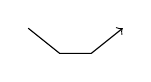
\begin{tikzpicture}[scale=0.4]
		\draw[->] (0, 0.8) -- (1, 0) -- (2, 0) -- (3, 0.8);
	\end{tikzpicture}
	tidak bergantung pada struktur penjumlahan pada himpunan-himpunan $\Hom$.
	Komposisi itu hanya melibatkan produk hingga dan koproduk hingga dalam
	kategori, termasuk kasus khususnya berupa objek nol, serta
	morfisme-morfisme kanonik yang terkait dengannya.

	Untuk (iii), ingat bahwa semua produk hingga (atau koproduk hingga) dapat
	dibentuk dari objek nol dan biproduk $\oplus$.

	Jika $(F,G)$ merupakan pasangan adjoin, maka $F$ mempertahankan
	$\varinjlim$, sedangkan $G$ mempertahankan $\varprojlim$; lihat
	\cite[Teorema 2.8.12]{Li1}. Di sisi lain, ekuivalensi mempertahankan semua
	limit. Karena itu, (iv) dan (v) keduanya merupakan kasus khusus dari (ii).
\end{bukti}

% segment-id: o014.li2.chapter1.additive-categories-kernels-cokernels.p010
Sesungguhnya, deskripsi penjumlahan dalam
Proposisi~\ref{prop:additive-cat-addition} menunjukkan bahwa ``keaditifan''
suatu kategori aditif $\mathcal{C}$ merupakan sifat dari kategori
$\mathcal{C}$, bukan struktur tambahan.

% segment-id: o014.li2.chapter1.additive-categories-kernels-cokernels.d002
\begin{definisi}
	\index{kernel (kernel)} \index[sym1]{kerf@$\Ker(f)$}
	\index{kokernel (cokernel)}\index[sym1]{cokerf@$\Coker(f)$}
	Misalkan $\mathcal{C}$ merupakan kategori-$\cate{Ab}$ yang mempunyai objek
	nol, dan $f: X \to Y$ suatu morfisme dalam $\mathcal{C}$.
	% segment-id: o014.li2.chapter1.additive-categories-kernels-cokernels.l006
	\begin{itemize}
		% segment-id: o014.li2.chapter1.additive-categories-kernels-cokernels.i014
		\item Jika penyama $\Ker(f,0)$ ada, maka $\Ker(f):=\Ker(f,0)$ beserta
		$\Ker(f) \hookrightarrow X$ disebut \emph{kernel} dari $f$.
		% segment-id: o014.li2.chapter1.additive-categories-kernels-cokernels.i015
		\item Jika kopenyama $\Coker(f,0)$ ada, maka $\Coker(f):=\Coker(f,0)$
		beserta $Y \twoheadrightarrow \Coker(f)$ disebut \emph{kokernel} dari
		$f$.
	\end{itemize}
	Secara khusus, menurut definisi kedua komposisi $\Ker(f) \to X \to Y$
	dan $X \to Y \to \Coker(f)$ sama dengan $0$.
\end{definisi}

% segment-id: o014.li2.chapter1.additive-categories-kernels-cokernels.p011
Terdapat beberapa sudut pandang yang saling melengkapi mengenai kernel dan
kokernel.
% segment-id: o014.li2.chapter1.additive-categories-kernels-cokernels.l007
\begin{itemize}
	% segment-id: o014.li2.chapter1.additive-categories-kernels-cokernels.i016
	\item Pertama, tinjau $\Ker(f)$. Untuk setiap morfisme $g: T \to X$ dengan
	$fg=0$,\footnote{Catatan penerjemah: teks sumber mengatakan ``untuk setiap
	morfisme'' tanpa mencantumkan syarat $fg=0$ dan, secara dual, $hf=0$.
	Kedua syarat itu dipulihkan di sini karena tepat merupakan hipotesis
	penyama dan kopenyama; lihat koreksi O014-C006.} komposisi
	$T \xrightarrow{g} X \xrightarrow{0} Y$ tentu sama dengan $0$.
	Karena itu, sifat universal $\Ker(f)=\Ker(f,0)$ sebagai penyama dapat
	dinyatakan oleh diagram komutatif
	% segment-id: o014.li2.chapter1.additive-categories-kernels-cokernels.g007
	\[\begin{tikzcd}
		& T \arrow[dashrightarrow, ld, "{\exists! g'}"'] \arrow[d, "g"] \arrow[rd, "0"] & \\
		\Ker(f) \arrow[r] & X \arrow[r, "f"'] & Y .
	\end{tikzcd}\]
	% segment-id: o014.li2.chapter1.additive-categories-kernels-cokernels.i017
	\item Tinjau $\Coker(f)$. Untuk setiap morfisme $h: Y \to T$ dengan
	$hf=0$, komposisi $X \xrightarrow{0} Y \xrightarrow{h} T$ tentu sama dengan
	$0$. Karena itu,
	sifat universal $\Coker(f)=\Coker(f,0)$ sebagai kopenyama dapat dinyatakan
	oleh diagram komutatif
	% segment-id: o014.li2.chapter1.additive-categories-kernels-cokernels.g008
	\[\begin{tikzcd}
		X \arrow[r, "f"] \arrow[rd, "0"'] & Y \arrow[r] \arrow[d, "h"] & \Coker(f) \arrow[dashrightarrow, ld, "{\exists! h'}"] . \\
		& T &
	\end{tikzcd}\]
	% segment-id: o014.li2.chapter1.additive-categories-kernels-cokernels.i018
	\item Kedua konstruksi di atas jelas saling dual:
	$\Coker(f)=\Ker(f^{\opp})$ dan $\Ker(f)=\Coker(f^{\opp})$.
\end{itemize}

% segment-id: o014.li2.chapter1.additive-categories-kernels-cokernels.p012
Karena morfisme yang terfaktorkan melalui objek nol tepat merupakan morfisme
$0$, sifat universal tersebut juga mempunyai karakterisasi melalui diagram
tarik balik dan dorong keluar. Pembaca dipersilakan memverifikasi langsung:

% segment-id: o014.li2.chapter1.additive-categories-kernels-cokernels.g009
\begin{equation}\label{eqn:Ker-Coker-triangles}
	\begin{tikzcd}
		\Ker(f) \arrow[phantom, r, "\simeq" description] & X \dtimes{Y} 0 \arrow[r] \arrow[d] \arrow[phantom, rd, "\Box" description] & X \arrow[d, "f"] \\
		& 0 \arrow[r] & Y
	\end{tikzcd} \qquad \begin{tikzcd}
		X \arrow[r, "f"] \arrow[d] & Y \arrow[d] & \\
		0 \arrow[r] & Y \dsqcup{X} 0 \arrow[phantom, lu, "\boxplus" description] & \Coker(f) \arrow[phantom, l, "\simeq" description] .
\end{tikzcd}\end{equation}

% segment-id: o014.li2.chapter1.additive-categories-kernels-cokernels.r001
\begin{catatan}\label{rem:equalizer-Ker}
	Penyama umum $\Ker(f,g)$ dapat direduksi menjadi kernel di atas. Tinjau
	morfisme-morfisme
	% segment-id: o014.li2.chapter1.additive-categories-kernels-cokernels.g010
	\[\begin{tikzcd}
	T \arrow[r, "h"] & X \arrow[r, yshift=0.2em, "f"] \arrow[r, yshift=-0.2em, "g"'] & Y
	\end{tikzcd}, \]
	Syarat $fh=gh$ ekuivalen dengan $(f-g)h=0$, sehingga langsung diperoleh
	$\Ker(f,g)=\Ker(f-g,0)=:\Ker(f-g)$. Secara dual,
	$\Coker(f,g)=\Coker(f-g,0)=:\Coker(f-g)$.
\end{catatan}

% segment-id: o014.li2.chapter1.additive-categories-kernels-cokernels.p013
Mulai sekarang, kita terutama meninjau kasus ketika $\mathcal{C}$ merupakan
kategori aditif.

% segment-id: o014.li2.chapter1.additive-categories-kernels-cokernels.pr003
\begin{proposisi}\label{prop:Ker-Coker-composite}
	Untuk morfisme-morfisme $X \xrightarrow{f} Y \xrightarrow{g} Z$ dalam
	kategori aditif $\mathcal{C}$, terdapat diagram komutatif
	% segment-id: o014.li2.chapter1.additive-categories-kernels-cokernels.g011
	\[\begin{tikzcd}[row sep=small, column sep=small]
		\Ker(gf) \arrow[rr, "\sim"] \arrow[hookrightarrow, rd] & & X \dtimes{Y} \Ker(g) \arrow[hookrightarrow, ld] \\
		& X &
	\end{tikzcd} \quad \begin{tikzcd}[row sep=small, column sep=small]
		Z \dsqcup{Y} \Coker(f) \arrow[rr, "\sim"] & & \Coker(gf) \\
		& Z \arrow[twoheadrightarrow, lu] \arrow[twoheadrightarrow, ru] &
	\end{tikzcd}\]
	di mana $X \dtimes{Y} \Ker(g) \to X$ (atau
	$Z \to Z \dsqcup{Y} \Coker(f)$) merupakan morfisme kanonik produk serat
	(atau koproduk serat),\footnote{Catatan penerjemah: teks sumber
	menulis ``koproduk'', tetapi objek yang ditampilkan adalah koproduk serat
	$Z \dsqcup{Y} \Coker(f)$ dan bukti berikutnya memakai dualitas terhadap
	produk serat; lihat koreksi O014-C005.} dengan ketentuan bahwa $\Ker$,
	$\Coker$, dan semua limit yang disebutkan ada.
\end{proposisi}

% segment-id: o014.li2.chapter1.additive-categories-kernels-cokernels.pf004
\begin{bukti}
	Berdasarkan \eqref{eqn:Ker-Coker-triangles}, pembentukan produk serat secara
	bertahap memberikan isomorfisme kanonik
	$\Ker(gf) \simeq X \dtimes{Z} 0 \simeq
	X \dtimes{Y} (Y \dtimes{Z} 0) \simeq X \dtimes{Y} \Ker(g)$.
	Dualitas memberikan kasus $\Coker(gf)$.
\end{bukti}

% segment-id: o014.li2.chapter1.additive-categories-kernels-cokernels.p014
Funktorialitas penyama dan kopenyama menginduksi funktorialitas kernel dan
kokernel. Konstruksi ini dicirikan oleh diagram komutatif berikut:

% segment-id: o014.li2.chapter1.additive-categories-kernels-cokernels.g012
\begin{equation}\label{eqn:Ker-Coker-functoriality}\begin{tikzcd}
		\Ker(f) \arrow[r] \arrow[dashrightarrow, d, "\exists!"'] & X \arrow[d, "a"'] \arrow[r, "f"] & Y \arrow[d, "b"] \\
		\Ker(g) \arrow[r] & X' \arrow[r, "g"'] & Y'
	\end{tikzcd} \qquad \begin{tikzcd}
		X \arrow[d, "a"'] \arrow[r, "f"] & Y \arrow[d, "b"] \arrow[r] & \Coker(f) \arrow[dashrightarrow, d, "\exists!"'] \\
		X' \arrow[r, "g"'] & Y' \arrow[r] & \Coker(g) .
\end{tikzcd}\end{equation}

% segment-id: o014.li2.chapter1.additive-categories-kernels-cokernels.p015
Hasil berikut menunjukkan bahwa tarik balik (atau dorong keluar)
mempertahankan kernel (atau kokernel).

% segment-id: o014.li2.chapter1.additive-categories-kernels-cokernels.pr004
\begin{proposisi}\label{prop:pull-back-ker}
	Jika diagram dalam kategori aditif $\mathcal{C}$
	% segment-id: o014.li2.chapter1.additive-categories-kernels-cokernels.g013
	\[\begin{tikzcd}
		X \arrow[r, "f"] \arrow[d, "a"'] & Y \arrow[d, "b"] \\
		X' \arrow[r, "g"'] & Y'
	\end{tikzcd}\]
	merupakan diagram tarik balik (atau dorong keluar), maka morfisme
	$\Ker(f) \to \Ker(g)$ (atau $\Coker(f) \to \Coker(g)$) dalam
	\eqref{eqn:Ker-Coker-functoriality} merupakan isomorfisme, dengan ketentuan
	bahwa $\Ker$ dan $\Coker$ yang dibicarakan ada.
\end{proposisi}

% segment-id: o014.li2.chapter1.additive-categories-kernels-cokernels.pf005
\begin{bukti}
	Dengan dualitas, cukup dibahas kasus tarik balik. Untuk setiap objek $T$,
	sifat universal memberikan
	% segment-id: o014.li2.chapter1.additive-categories-kernels-cokernels.a001
	\begin{align*}
		\Hom(T, \Ker(f)) & \simeq \Ker\left[ \Hom(T, X) \to \Hom(T, Y) \right] \\
		& \simeq \Ker\left[ \Hom(T, Y) \dtimes{\Hom(T, Y')} \Hom(T, X') \to \Hom(T, Y) \right] \\
		& = \Ker\left[ \Hom(T, X') \to \Hom(T, Y') \right] \simeq \Hom(T, \Ker(g)),
	\end{align*}
	dengan setiap panah bersifat kanonik. Lema Yoneda kemudian memberikan
	$\Ker(f) \rightiso \Ker(g)$; lihat tinjauan dalam
	Teorema~\sourcecrossref{prop:Yoneda}{A.1.1}.
\end{bukti}

% segment-id: o014.li2.chapter1.additive-categories-kernels-cokernels.lm001
\begin{lema}\label{prop:mono-epi-ker-coker}
	Misalkan $\mathcal{C}$ merupakan kategori aditif dan $f: X \to Y$ suatu
	morfisme dalam $\mathcal{C}$. Maka:
	% segment-id: o014.li2.chapter1.additive-categories-kernels-cokernels.l008
	\begin{enumerate}[(i)]
		% segment-id: o014.li2.chapter1.additive-categories-kernels-cokernels.i019
		\item $f$ merupakan monomorfisme (atau epimorfisme) jika dan hanya jika
		$\Ker(f)=0$ (atau $\Coker(f)=0$);
		% segment-id: o014.li2.chapter1.additive-categories-kernels-cokernels.i020
		\item $f$ merupakan morfisme nol jika dan hanya jika
		$\Ker(f) \rightiso X$, dan ini juga ekuivalen dengan
		$Y \rightiso \Coker(f)$;
		% segment-id: o014.li2.chapter1.additive-categories-kernels-cokernels.i021
		\item Diberikan $k: Y \to Z$ (atau $k': W \to X$), terdapat secara unik
		diagram komutatif berikut:
		% segment-id: o014.li2.chapter1.additive-categories-kernels-cokernels.g014
		\[\begin{tikzcd}[row sep=small, column sep=small]
		\Ker(kf) \arrow[rd] & & \Ker(f) \arrow[ld] \arrow[hookrightarrow, ll, "\exists !"'] \\
		& X &
		\end{tikzcd} \quad \text{atau} \quad
		\begin{tikzcd}[row sep=small, column sep=small]
		\Coker(fk') \arrow[twoheadrightarrow, rr, "\exists !"] & & \Coker(f) \\
		& Y \arrow[lu] \arrow[ru] &
		\end{tikzcd}\]
		dengan ketentuan bahwa kernel (atau kokernel) yang dibicarakan ada. Jika
		$k$ merupakan monomorfisme (atau $k'$ merupakan epimorfisme), maka
		$\Ker(f) \rightiso \Ker(kf)$ (atau
		$\Coker(fk') \rightiso \Coker(f)$).
	\end{enumerate}
\end{lema}

% segment-id: o014.li2.chapter1.additive-categories-kernels-cokernels.pf006
\begin{bukti}
	Pertama, tinjau (i). Berdasarkan dualitas, cukup dibahas kasus
	monomorfisme. Menurut definisi, $f$ merupakan monomorfisme jika dan hanya
	jika untuk setiap pasangan morfisme $g_1,g_2: T \to X$ berlaku
	$f(g_1-g_2)=0 \iff g_1-g_2=0$. Ini setara dengan pernyataan bahwa untuk
	setiap $g: T \to X$, berlaku $fg=0$ jika dan hanya jika $g$ terfaktorkan
	sebagai $T \to 0 \to X$. Pernyataan terakhir ini tepat menyatakan bahwa
	objek nol memenuhi sifat universal $\Ker(f)$.

	Untuk (ii), secara serupa cukup dibuktikan
	$f=0 \iff \Ker(f) \rightiso X$. Akan tetapi,
	$\Ker(f)=\Ker(f,0)$, sehingga ekuivalensi yang diinginkan langsung
	mengikuti definisi penyama.

	Untuk (iii), sekali lagi cukup ditinjau kasus $\Ker$:
	% segment-id: o014.li2.chapter1.additive-categories-kernels-cokernels.g015
	\[\begin{tikzcd}[column sep=small]
		\left\{ g \in \Hom(T, X): fg=0 \right\} \arrow[phantom, r, "\subset" description] & \left\{ g \in \Hom(T, X): kfg=0 \right\} \\
		\Hom(T, \Ker(f)) \arrow[u, "1:1"] & \Hom(T, \Ker(kf)) \arrow[u, "1:1"']
	\end{tikzcd}\]
	Jika $k$ merupakan monomorfisme, inklusi pada baris pertama merupakan
	kesamaan. Terapkan Lema Yoneda untuk menyelesaikan pembuktian.
\end{bukti}

% segment-id: o014.li2.chapter1.additive-categories-kernels-cokernels.p016
Dalam kategori aditif, citra dan kocitra yang diperkenalkan dalam
Definisi~\ref{def:Im-Coim} mempunyai deskripsi sederhana.

% segment-id: o014.li2.chapter1.additive-categories-kernels-cokernels.pr005
\begin{proposisi}\label{prop:Im-Coim-additive}
	\index{citra (image)}\index{kocitra (coimage)}
	\index[sym1]{imf@$\Image(f)$}\index[sym1]{coimf@$\Coim(f)$}
	Misalkan $f: X \to Y$ merupakan morfisme dalam kategori aditif
	$\mathcal{C}$. Maka terdapat isomorfisme kanonik
	% segment-id: o014.li2.chapter1.additive-categories-kernels-cokernels.a002
	\begin{align*}
		\Image(f) & \simeq \Ker\left[ Y \to \Coker(f) \right] \hookrightarrow Y, \\
		\Coim(f) & \simeq \Coker\left[ \Ker(f) \to X \right] \twoheadleftarrow X ;
	\end{align*}
	dengan ketentuan bahwa kernel dan kokernel yang dibicarakan ada.
\end{proposisi}

% segment-id: o014.li2.chapter1.additive-categories-kernels-cokernels.pf007
\begin{bukti}
	Berdasarkan dualitas, cukup ditinjau $\Image(f)$. Ambil morfisme kanonik
	$i_1,i_2: Y \to Y \dsqcup{X} Y$. Dengan menerapkan Lema Yoneda, cukup
	dibuktikan, untuk setiap $T \in \Obj(\mathcal{C})$, bahwa
	% segment-id: o014.li2.chapter1.additive-categories-kernels-cokernels.q008
	\begin{multline*}
		\Hom\left( T, \Image(f) \right) = \left\{ h: T \to Y \;\middle|\; i_1 h = i_2 h \right\} \\
		= \left\{ \begin{array}{r|l}
			h: T \to Y & \forall S \in \Obj(\mathcal{C}),\; \forall s_1, s_2: Y \to S, \\
			& s_1 f = s_2 f \implies s_1 h = s_2 h
		\end{array}\right\} \\
		\xlongequal{s := s_1 - s_2} \left\{ \begin{array}{r|l}
			h: T \to Y & \forall S \in \Obj(\mathcal{C}),\; \forall s: Y \to S, \\
			& s f = 0 \implies sh = 0
		\end{array}\right\} \\
		= \left\{ \begin{array}{r|l}
			h: T \to Y & T \xrightarrow{h} Y \twoheadrightarrow \Coker(f) \\
			& \text{komposisinya adalah}\; 0
		\end{array}\right\}
		\leftiso \Hom\left( T, \Ker\left[ Y \to \Coker(f) \right] \right).
	\end{multline*}
	Kesamaan pertama di atas berasal dari
	$\Image(f):=\Ker(i_1,i_2)$. Untuk kesamaan kedua, mula-mula tuliskan ulang
	syarat pada $h$ sebagai $s'i_1h=s'i_2h$ bagi setiap
	$s': Y \dsqcup{X} Y \to S$, lalu gunakan sifat universal koproduk serat
	% segment-id: o014.li2.chapter1.additive-categories-kernels-cokernels.a003
	\begin{align*}
		\Hom\left( Y \dsqcup{X} Y, S \right) & \xrightarrow{1:1} \Hom(Y,S) \dtimes{\Hom(X,S)} \Hom(Y,S) \\
		s' & \longmapsto \left( s' i_1, s' i_2 \right) =: (s_1, s_2).
	\end{align*}
	Kesamaan keempat diperoleh dari sifat universal kokernel, sehingga cukup
	diambil $S=\Coker(f)$.
\end{bukti}

% segment-id: o014.li2.chapter1.additive-categories-kernels-cokernels.p017
Contoh paling sederhana terjadi ketika $f$ merupakan morfisme nol. Dalam hal
ini, Lema~\ref{prop:mono-epi-ker-coker} (ii) memberikan
$\Image(f)=0=\Coim(f)$.

% segment-id: o014.li2.chapter1.additive-categories-kernels-cokernels.e002
\begin{contoh}\label{eg:strict-morphism}
	Sebagai kelanjutan pembahasan pada Contoh~\ref{eg:additive-category},
	pertama-tama kita tinjau kategori $R\dcate{Mod}$. Homomorfisme modul
	$f: A \to B$ selalu mempunyai
	kernel dan kokernel, yang secara klasik diberikan oleh
	$\Ker(f)=f^{-1}(0)$ dan
	$\Coker(f)=B/\{f(a):a \in A\}$. Langsung dari definisi, $\Image(f)$ adalah
	citra $f$ dalam pengertian teori himpunan, sedangkan
	$\Coim(f)=A/\Ker(f)$. Morfisme kanonik
	$\Coim(f) \to \Image(f)$ dalam \eqref{eqn:strict-morphism} tepat
	merupakan isomorfisme kanonik dalam teori modul
	$A/\Ker(f) \rightiso \Image(f)$. Karena itu, semua morfisme dalam
	$R\dcate{Mod}$ bersifat ketat.

	Selanjutnya, tinjau kategori aditif $\cate{Ban}_{\CC}$ dari
	Contoh~\ref{eg:additive-category}. Kernel dari pemetaan linear kontinu
	$f: X \to Y$ adalah $\Ker(f)=f^{-1}(0)$ seperti biasa, dan tetap merupakan
	ruang Banach. Di sisi lain,
	$\Coker(f)=Y/\overline{\left\{f(x):x \in X\right\}}$ dilengkapi dengan
	norma kuosien. Dalam hal ini, morfisme \eqref{eqn:strict-morphism} menjadi
	% segment-id: o014.li2.chapter1.additive-categories-kernels-cokernels.g016
	\[\begin{tikzcd}[row sep=small, column sep=small]
	\Coim(f) \arrow[equal, r] & X/f^{-1}(0) \arrow[r] & \overline{\left\{ f(x): x \in X \right\}} \arrow[equal, r] & \Image(f) \\
	& x + f^{-1}(0) \arrow[mapsto, r] \arrow[phantom, u, "\in" description, sloped] & f(x) \arrow[phantom, u, "\in" description, sloped] &
	\end{tikzcd}\]
	Ruang di sebelah kanan dilengkapi dengan topologi terinduksi dari $Y$,
	sedangkan ruang di sebelah kiri dilengkapi dengan topologi kuosien dari
	$X$. Misalkan
	$f: X \to Y$ merupakan pemetaan linear kontinu dan injektif antara ruang
	Banach, dengan citra padat tetapi tidak surjektif. Dalam keadaan ini,
	$\Coim(f)=X \to Y=\Image(f)$ bukan isomorfisme. Jadi,
	$\cate{Ban}_{\CC}$ mempunyai morfisme yang tidak ketat.
\end{contoh}
